A NASNet modell sb-photothemes-imagenet114 adathalmazon teljes tanítással történt tesztelésének eredménye. Lásd a soron következő ábrákat és táblázatokat a mérések eredményeihez.

\subsubsection{NASNet teljes tanítás folyamata}
\begin{itemize} 
	\item Epoch 1/3 - train: 2259/2259 [11:55<00:00,  3.16it/s]
	\item Epoch 1/3 - val: 282/282 [00:23<00:00, 12.21it/s]
	\item Epoch 1: Train loss=1.2301, acc=0.6617 Val loss=0.9508, acc=0.7256
	\item Epoch 2/3 - train: 2259/2259 [11:54<00:00,  3.16it/s]
	\item Epoch 2/3 - val: 282/282 [00:23<00:00, 12.17it/s]
	\item Epoch 2: Train loss=0.6347, acc=0.8083 Val loss=0.9009, acc=0.7561
	\item Epoch 3/3 - train: 2259/2259 [11:55<00:00,  3.16it/s]
	\item Epoch 3/3 - val: 282/282 [00:23<00:00, 12.20it/s]
	\item Epoch 3: Train loss=0.3706, acc=0.8858 Val loss=0.9542, acc=0.7598
\end{itemize}

\subsubsection{NASNet teljes tanítás folyamata}
  \begin{figure}[H]
    \centering
    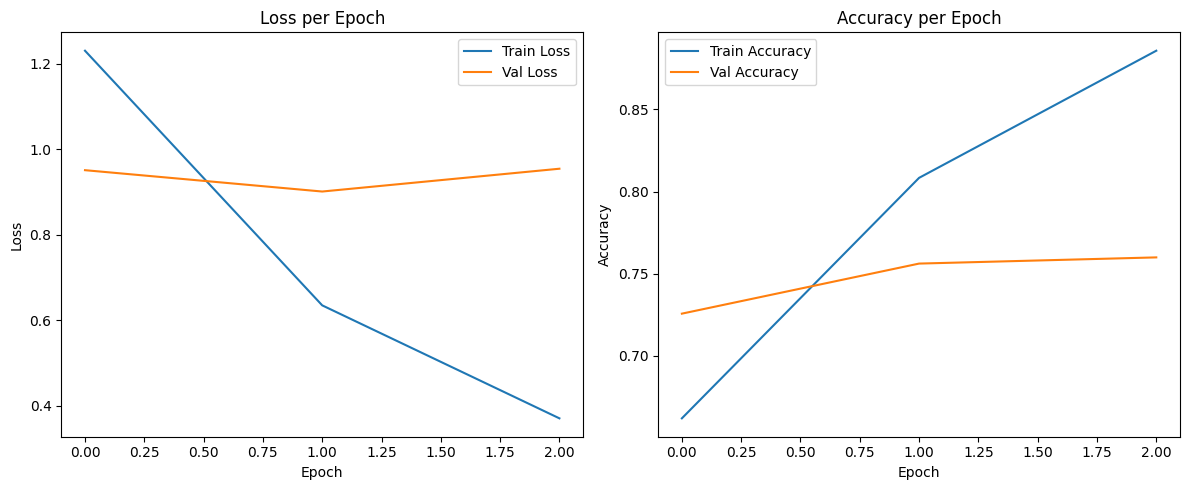
\includegraphics[width=1.0\textwidth]{images/phase02/NASNet_learning_curve.png}
    \caption{NASNet teljes tanítás utáni sima Confusion Mátrix}
    \label{fig:phase02_NASNet_learning_curves}
  \end{figure}

\subsubsection{NASNet teljes tanítás utáni eredményei}
  \begin{center}
  \begin{longtable}{l c}
  \caption{NASNet teljes tanítás utáni vizsgálati eredményei} \label{tab:phase02_NASNet} \\
  \toprule
  \textbf{Metrika} & \textbf{Érték} \\
  \midrule
  \endfirsthead
  \toprule
  \textbf{Metrika} & \textbf{Érték} \\
  \midrule
  \endhead
  Top-1 Accuracy & 0.7626 \\
  Top-5 Accuracy & 0.9470 \\
  Precision & 0.7180 \\
  Recall & 0.6875 \\
  F1-score & 0.6955 \\
  Inference time & 25.11 sec \\
  \bottomrule
  \end{longtable}
  \end{center}

\subsubsection{NASNet eredményeinek összehasonlítása}
  \begin{center}
  \begin{longtable}{l c c}
  \caption{NASNet eredményeinek összehasonlítása} \label{tab:phase02_NASNet_compare} \\
  \toprule
  \textbf{Metrika} & \textbf{Pretrained} & \textbf{Fine-tuned} \\
  \midrule
  \endfirsthead
  \toprule
  \textbf{Metrika} & \textbf{Pretrained} & \textbf{Fine-tuned} \\
  \midrule
  \endhead
  Top-1 Accuracy  & 0.2820 & 0.7626 \\
  Top-5 Accuracy & 0.5408 & 0.9470 \\
  Precision & 0.3204 & 0.7180 \\
  Recall & 0.2799 & 0.6808 \\
  F1-score & 0.2696 & 0.6955 \\
  Inference time & 275.30 sec & 34.03 sec \\
  \bottomrule
  \end{longtable}
  \end{center}

\subsubsection{NASNet eredményeinek összehasonlítása}
  \begin{figure}[H]
    \centering
    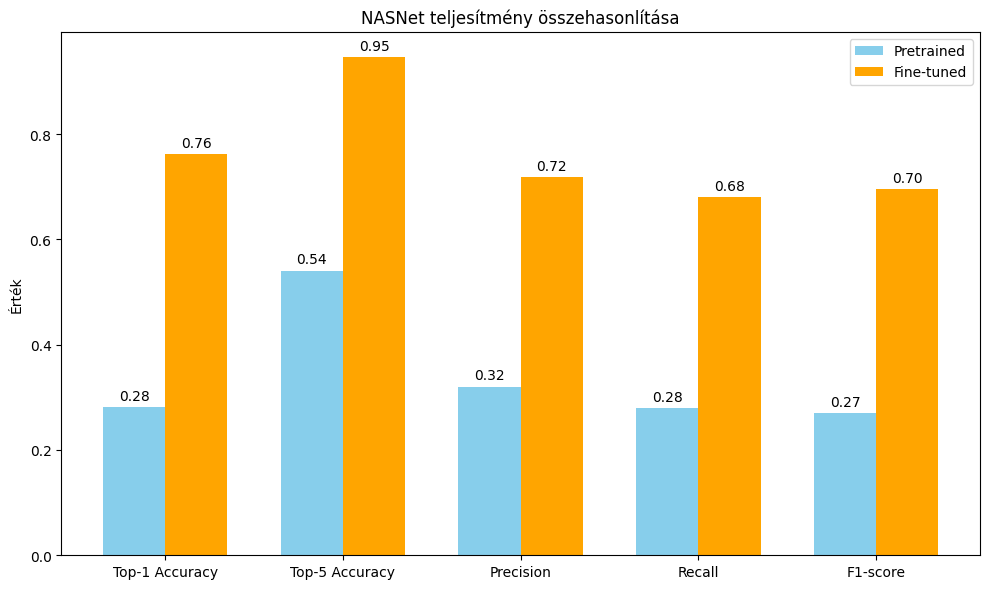
\includegraphics[width=1.0\textwidth]{images/phase02/NASNet_compare01.png}
    \caption{NASNet eredményeinek összehasonlítása}
    \label{fig:NASNet_compare01}
  \end{figure}

\subsubsection{NASNet eredményeinek összehasonlítása}
  \begin{figure}[H]
    \centering
    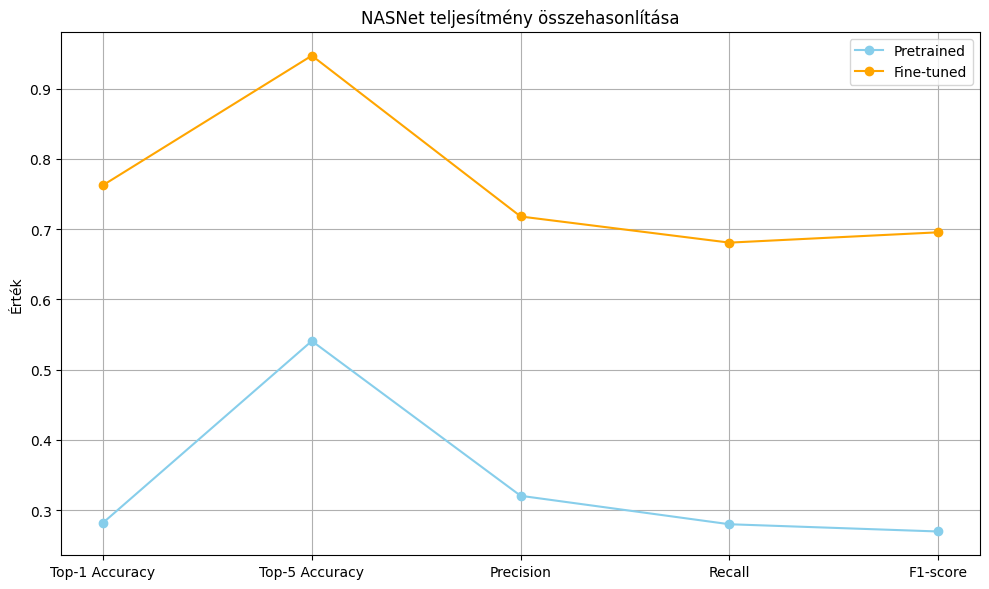
\includegraphics[width=1.0\textwidth]{images/phase02/NASNet_compare02.png}
    \caption{NASNet eredményeinek összehasonlítása}
    \label{fig:NASNet_compare02}
  \end{figure}

\subsubsection{NASNet teljes tanítás utáni sima Confusion Mátrix}
  \begin{figure}[H]
    \centering
    
\includegraphics[width=1.0\textwidth]{images/phase02/NASNet_basic_conf_mat.png}
    \caption{NASNet teljes tanítás utáni sima Confusion Mátrix}
    \label{fig:phase02_NASNet_basic_conf_mat}
  \end{figure}

  \subsubsection{NASNet Confusion Mátrixok összehasonlítása}
  \begin{figure}[H]
    \centering
    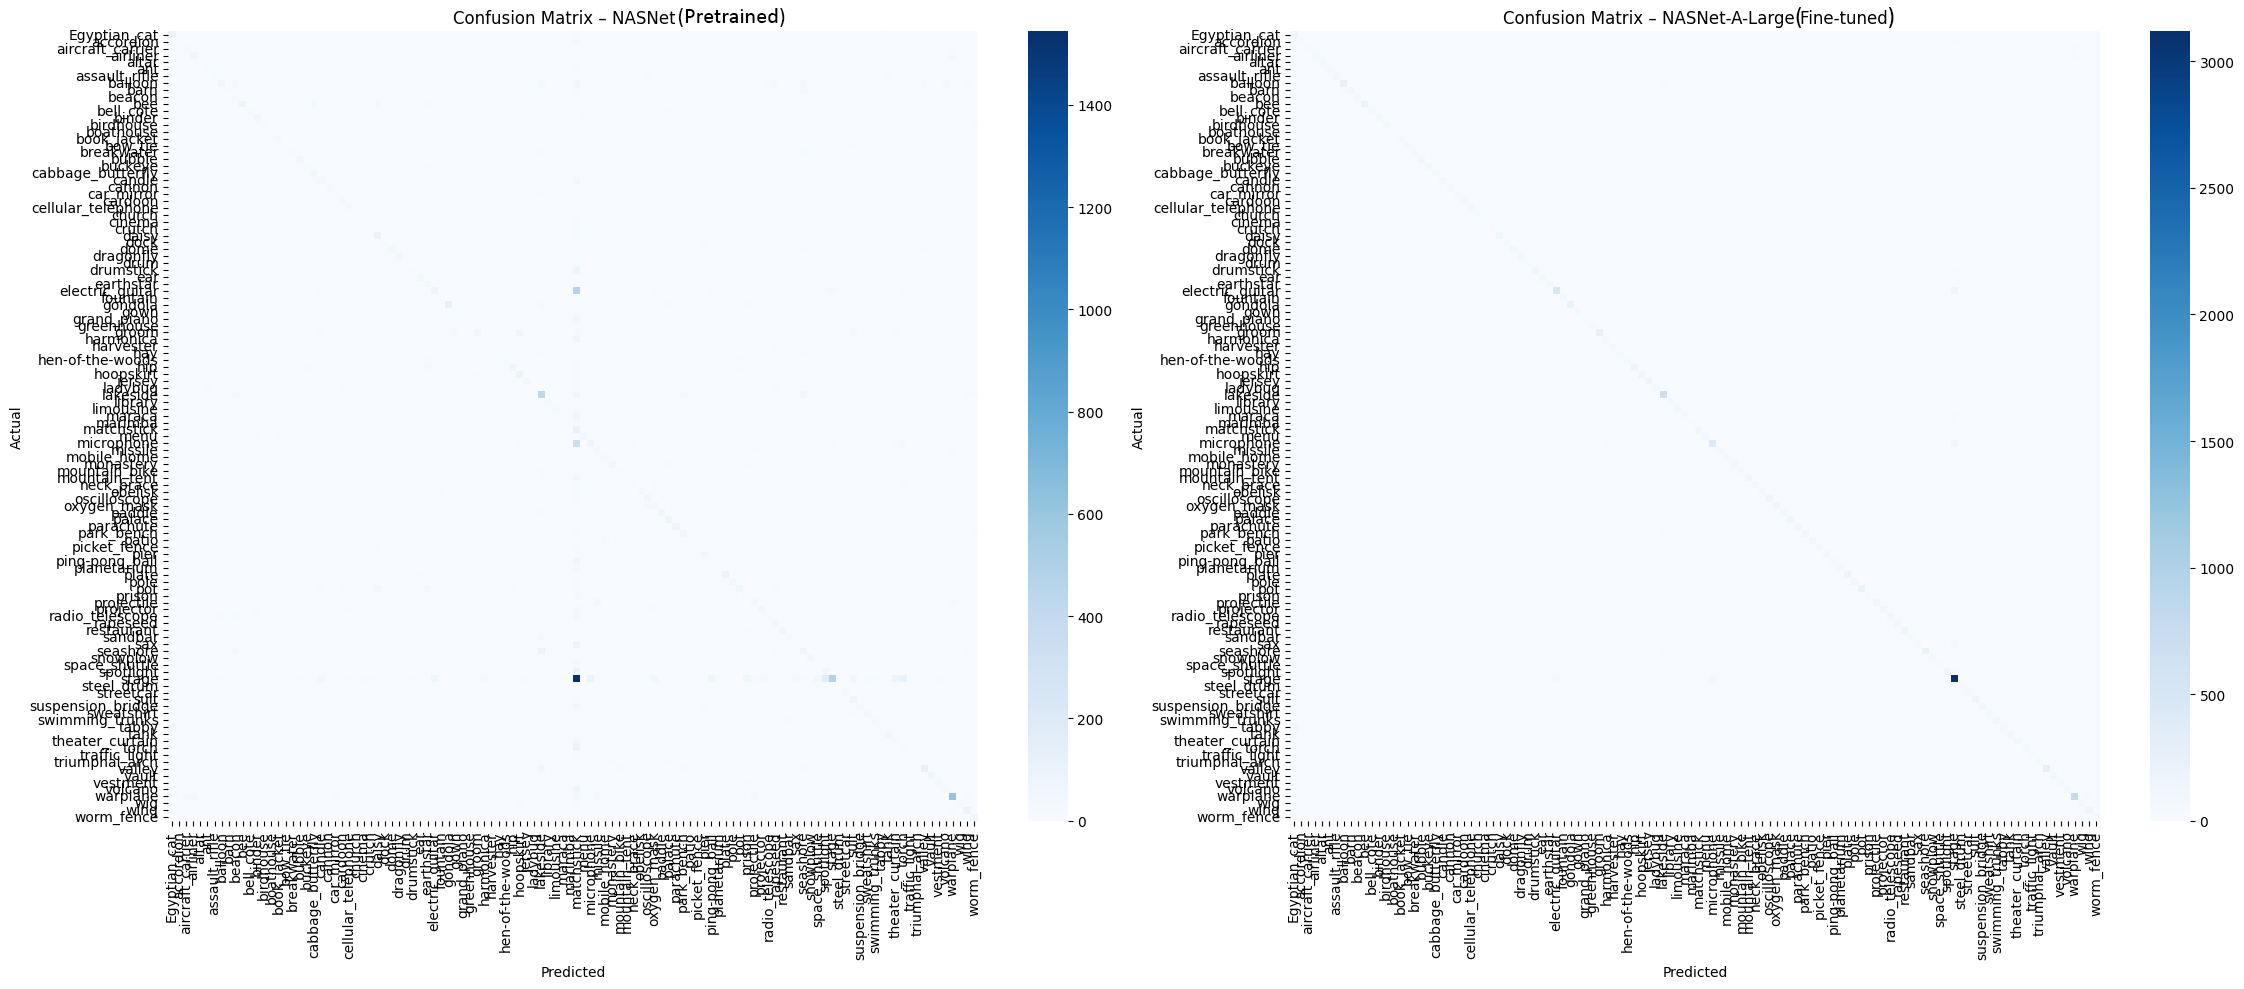
\includegraphics[width=1.0\textwidth]{images/phase02/NASNet_basic_conf_mat_compare.png}
    \caption{NASNet sima Confusion Mátrixok összehasonlítása}
    \label{fig:phase02_NASNet_basic_conf_mat_compare}
  \end{figure}

  \subsubsection{NASNet teljes tanítás utáni normalizált Confusion Mátrix}
  \begin{figure}[H]
    \centering
    
\includegraphics[width=1.0\textwidth]{images/phase02/NASNet_normalised_conf_mat.png}
    \caption{NASNet teljes tanítás utáni normalizált Confusion Mátrix}
    \label{fig:phase02_NASNet_normalised_conf_mat}
  \end{figure}

  \subsubsection{NASNet normalizált Confusion Mátrixok összehasonlítása}
  \begin{figure}[H]
    \centering
    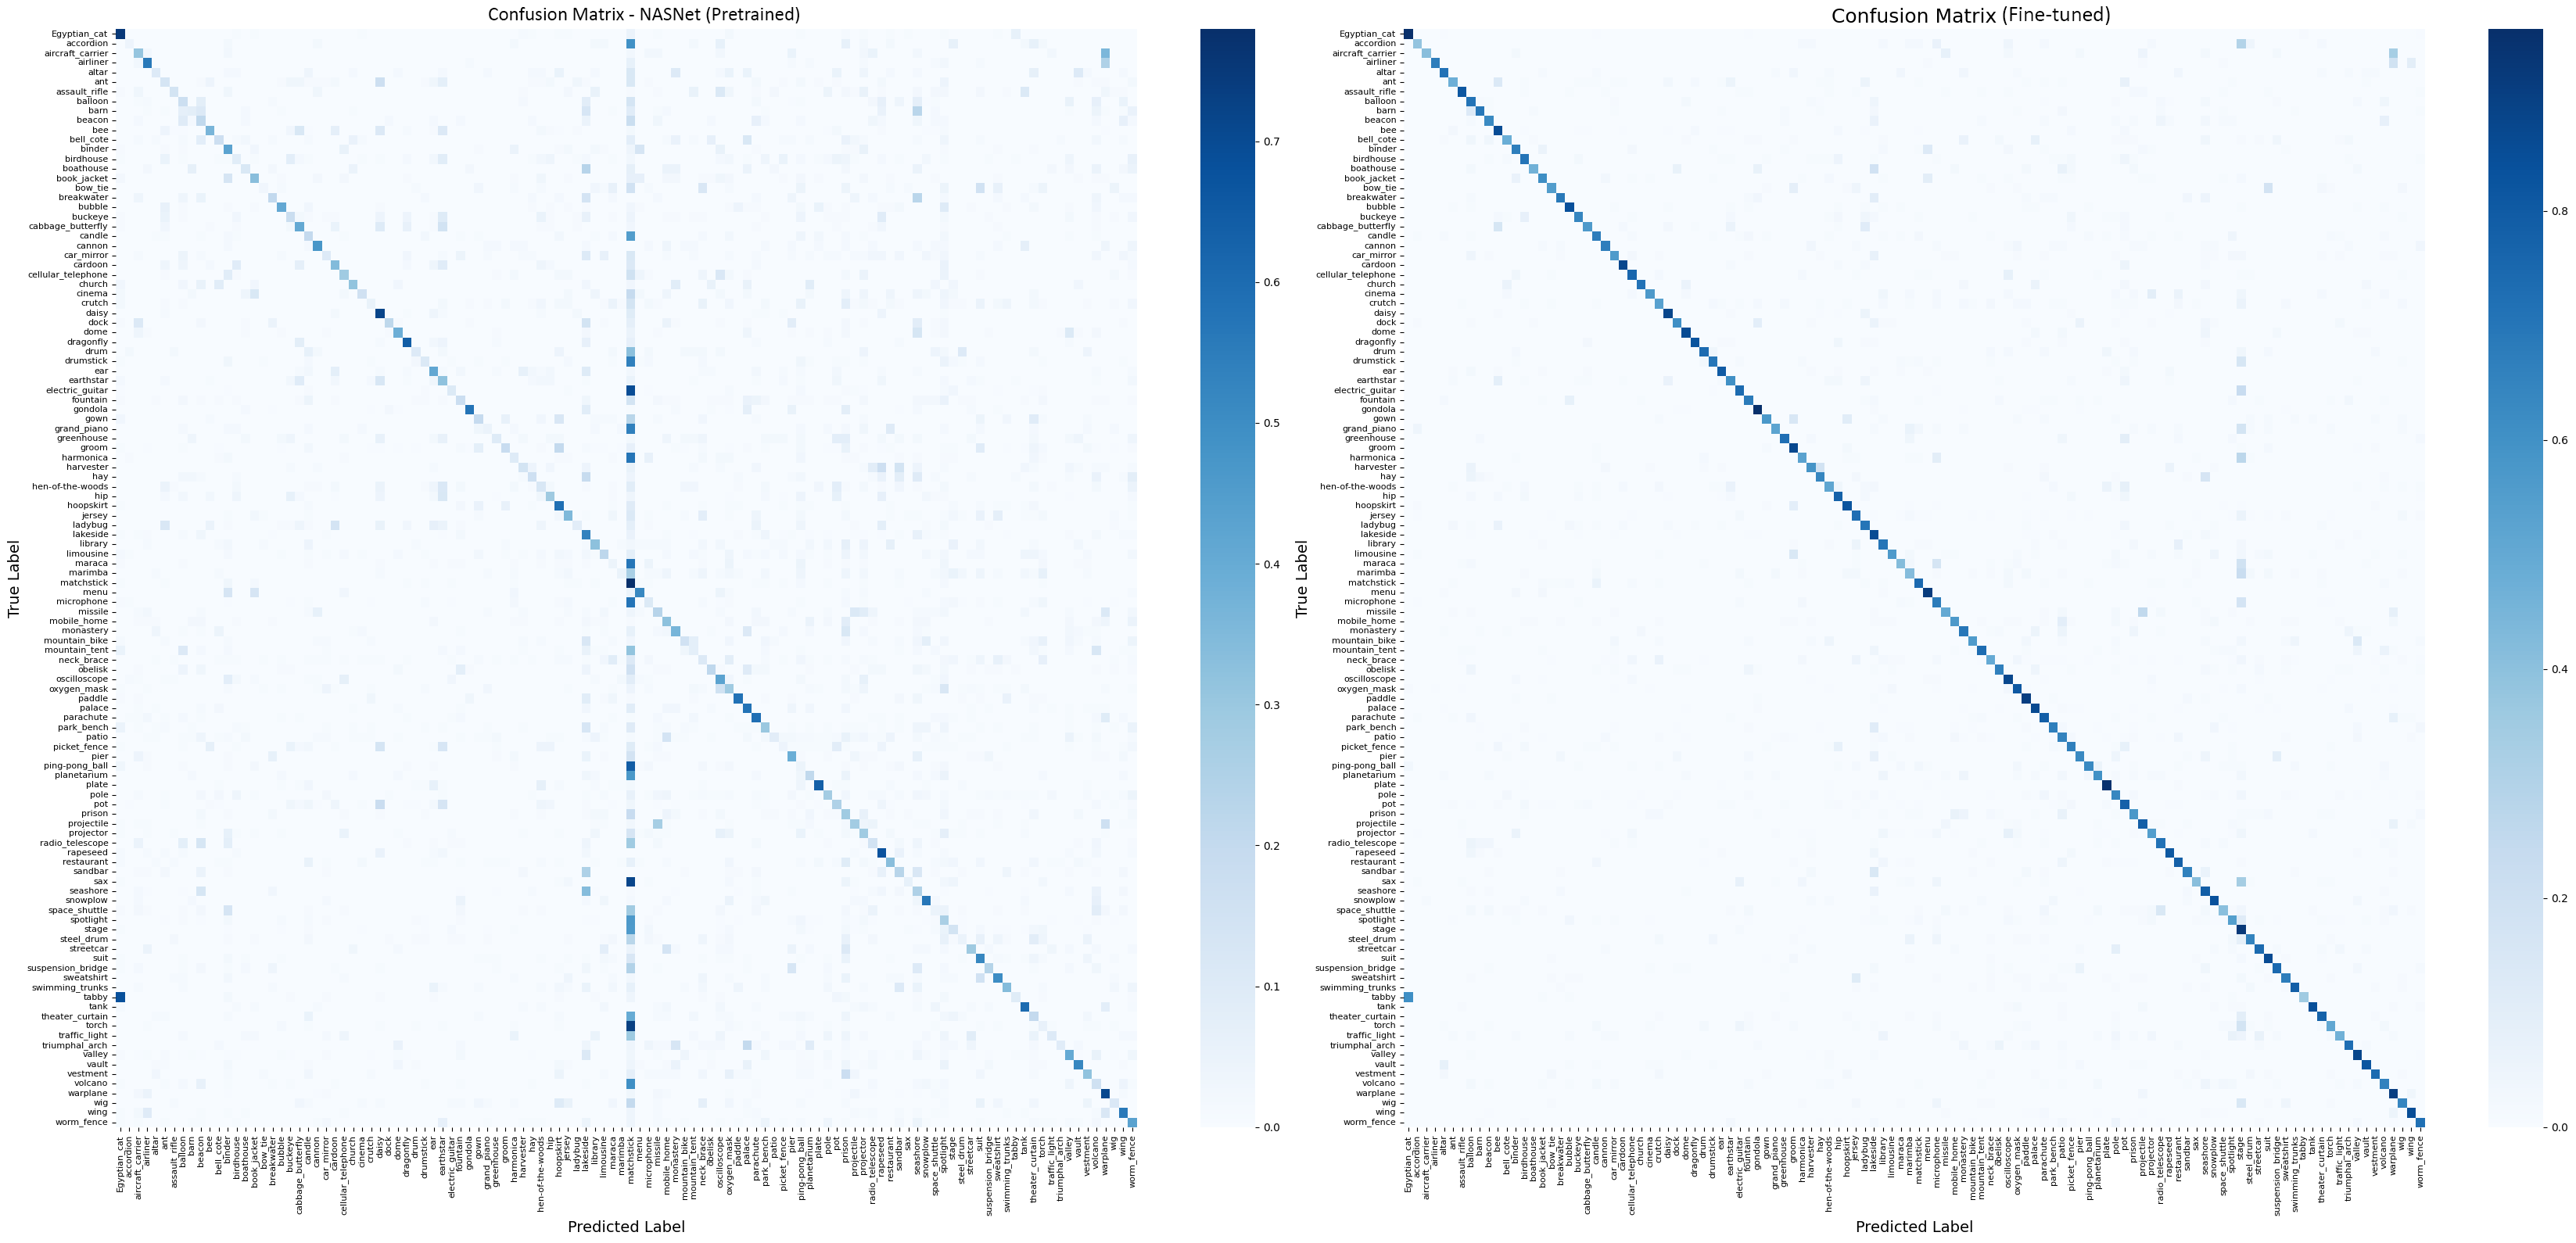
\includegraphics[width=1.0\textwidth]{images/phase02/NASNet_normalised_conf_mat_compare.png}
    \caption{NASNet normalizált Confusion Mátrixok összehasonlítása}
    \label{fig:phase02_NASNet_normalised_conf_mat_compare}
  \end{figure}

\subsubsection{NASNet teljes tanítás utáni részletes osztályonkénti metrikák}
  \begin{center}
\begin{longtable}{lllll}
\caption{NASNet teljes tanítás utáni részletes osztályonkénti metrikák}\label{tab:phase2_NASNet_class_table}\\
\toprule
class & precision & recall & f1-score & support \\
\midrule
\endfirsthead
\toprule
class & precision & recall & f1-score & support \\
\midrule
\endhead
airliner & 0.98 & 0.68 & 0.80 & 80 \\
tabby & 0.95 & 0.36 & 0.52 & 107 \\
warplane & 0.91 & 0.91 & 0.91 & 871 \\
tank & 0.90 & 0.85 & 0.87 & 78 \\
aircraft-carrier & 0.89 & 0.41 & 0.56 & 39 \\
dragonfly & 0.89 & 0.83 & 0.86 & 75 \\
gondola & 0.89 & 0.96 & 0.92 & 227 \\
vault & 0.89 & 0.82 & 0.85 & 104 \\
assault-rifle & 0.88 & 0.81 & 0.85 & 91 \\
daisy & 0.86 & 0.88 & 0.87 & 149 \\
mountain-tent & 0.86 & 0.74 & 0.79 & 121 \\
ping-pong-ball & 0.86 & 0.63 & 0.73 & 91 \\
plate & 0.86 & 0.95 & 0.90 & 143 \\
electric-guitar & 0.85 & 0.74 & 0.79 & 687 \\
stage & 0.85 & 0.92 & 0.89 & 3380 \\
cabbage-butterfly & 0.84 & 0.56 & 0.67 & 101 \\
cardoon & 0.84 & 0.87 & 0.86 & 55 \\
church & 0.83 & 0.71 & 0.77 & 35 \\
hoopskirt & 0.83 & 0.82 & 0.83 & 135 \\
swimming-trunks & 0.83 & 0.78 & 0.81 & 79 \\
lakeside & 0.82 & 0.86 & 0.84 & 801 \\
limousine & 0.82 & 0.56 & 0.67 & 119 \\
obelisk & 0.82 & 0.66 & 0.73 & 95 \\
valley & 0.81 & 0.88 & 0.84 & 295 \\
drumstick & 0.80 & 0.70 & 0.75 & 126 \\
ear & 0.80 & 0.80 & 0.80 & 80 \\
groom & 0.80 & 0.87 & 0.83 & 285 \\
barn & 0.79 & 0.69 & 0.74 & 111 \\
rapeseed & 0.79 & 0.81 & 0.80 & 77 \\
hip & 0.78 & 0.77 & 0.78 & 195 \\
suspension-bridge & 0.77 & 0.75 & 0.76 & 127 \\
worm-fence & 0.77 & 0.72 & 0.75 & 137 \\
bubble & 0.76 & 0.84 & 0.80 & 100 \\
dock & 0.76 & 0.61 & 0.68 & 84 \\
palace & 0.76 & 0.86 & 0.81 & 139 \\
park-bench & 0.76 & 0.67 & 0.71 & 144 \\
suit & 0.76 & 0.86 & 0.80 & 141 \\
vestment & 0.76 & 0.74 & 0.75 & 69 \\
balloon & 0.75 & 0.71 & 0.73 & 338 \\
matchstick & 0.75 & 0.75 & 0.75 & 127 \\
microphone & 0.75 & 0.68 & 0.71 & 596 \\
bee & 0.74 & 0.85 & 0.79 & 212 \\
bow-tie & 0.74 & 0.55 & 0.63 & 67 \\
buckeye & 0.74 & 0.64 & 0.69 & 101 \\
dome & 0.74 & 0.86 & 0.79 & 85 \\
greenhouse & 0.74 & 0.73 & 0.73 & 51 \\
oxygen-mask & 0.74 & 0.81 & 0.78 & 143 \\
breakwater & 0.73 & 0.69 & 0.71 & 58 \\
monastery & 0.73 & 0.70 & 0.71 & 112 \\
restaurant & 0.73 & 0.78 & 0.76 & 141 \\
cellular-telephone & 0.72 & 0.76 & 0.74 & 104 \\
gown & 0.72 & 0.58 & 0.64 & 66 \\
pot & 0.72 & 0.78 & 0.75 & 254 \\
wing & 0.72 & 0.85 & 0.78 & 148 \\
boathouse & 0.71 & 0.47 & 0.56 & 43 \\
book-jacket & 0.71 & 0.61 & 0.65 & 90 \\
neck-brace & 0.71 & 0.50 & 0.58 & 137 \\
pier & 0.71 & 0.63 & 0.67 & 97 \\
sandbar & 0.71 & 0.66 & 0.68 & 83 \\
bell-cote & 0.70 & 0.48 & 0.57 & 77 \\
jersey & 0.70 & 0.73 & 0.71 & 154 \\
mobile-home & 0.70 & 0.57 & 0.63 & 83 \\
oscilloscope & 0.70 & 0.87 & 0.78 & 143 \\
radio-telescope & 0.70 & 0.71 & 0.71 & 108 \\
triumphal-arch & 0.70 & 0.73 & 0.71 & 55 \\
cannon & 0.69 & 0.67 & 0.68 & 55 \\
drum & 0.69 & 0.73 & 0.71 & 49 \\
mountain-bike & 0.69 & 0.56 & 0.62 & 66 \\
seashore & 0.69 & 0.79 & 0.74 & 289 \\
spotlight & 0.69 & 0.54 & 0.61 & 202 \\
steel-drum & 0.69 & 0.65 & 0.67 & 84 \\
streetcar & 0.69 & 0.74 & 0.71 & 65 \\
torch & 0.69 & 0.51 & 0.59 & 116 \\
missile & 0.68 & 0.50 & 0.58 & 82 \\
projector & 0.68 & 0.55 & 0.61 & 157 \\
sweatshirt & 0.68 & 0.68 & 0.68 & 80 \\
Egyptian-cat & 0.67 & 0.96 & 0.79 & 145 \\
ant & 0.67 & 0.47 & 0.56 & 95 \\
binder & 0.67 & 0.67 & 0.67 & 105 \\
birdhouse & 0.67 & 0.71 & 0.69 & 116 \\
cinema & 0.67 & 0.57 & 0.62 & 51 \\
grand-piano & 0.66 & 0.52 & 0.58 & 63 \\
planetarium & 0.66 & 0.60 & 0.63 & 62 \\
earthstar & 0.65 & 0.60 & 0.62 & 121 \\
hen-of-the-woods & 0.65 & 0.51 & 0.57 & 105 \\
menu & 0.65 & 0.91 & 0.76 & 68 \\
paddle & 0.65 & 0.90 & 0.76 & 93 \\
parachute & 0.65 & 0.79 & 0.71 & 117 \\
picket-fence & 0.65 & 0.67 & 0.66 & 118 \\
theater-curtain & 0.65 & 0.78 & 0.71 & 80 \\
wig & 0.65 & 0.64 & 0.65 & 70 \\
altar & 0.64 & 0.71 & 0.67 & 59 \\
candle & 0.64 & 0.68 & 0.66 & 111 \\
crutch & 0.64 & 0.53 & 0.58 & 105 \\
hay & 0.64 & 0.64 & 0.64 & 73 \\
traffic-light & 0.64 & 0.47 & 0.54 & 58 \\
fountain & 0.63 & 0.68 & 0.66 & 92 \\
snowplow & 0.63 & 0.84 & 0.72 & 62 \\
harvester & 0.62 & 0.59 & 0.60 & 71 \\
sax & 0.62 & 0.41 & 0.49 & 112 \\
ladybug & 0.61 & 0.70 & 0.66 & 108 \\
prison & 0.60 & 0.57 & 0.59 & 101 \\
space-shuttle & 0.59 & 0.40 & 0.48 & 84 \\
volcano & 0.59 & 0.66 & 0.62 & 119 \\
beacon & 0.58 & 0.63 & 0.60 & 62 \\
car-mirror & 0.57 & 0.56 & 0.56 & 68 \\
projectile & 0.56 & 0.79 & 0.66 & 117 \\
patio & 0.55 & 0.65 & 0.60 & 144 \\
pole & 0.55 & 0.64 & 0.59 & 136 \\
library & 0.51 & 0.70 & 0.59 & 74 \\
harmonica & 0.50 & 0.53 & 0.51 & 100 \\
accordion & 0.49 & 0.38 & 0.43 & 47 \\
maraca & 0.49 & 0.42 & 0.46 & 90 \\
marimba & 0.39 & 0.42 & 0.40 & 79 \\
\midrule
accuracy &  &  & 0.76 & 18172 \\
macro-avg & 0.72 & 0.69 & 0.70 & 18172 \\
weighted-avg & 0.76 & 0.76 & 0.76 & 18172 \\
\bottomrule
\end{longtable}
\end{center}


\subsubsection{GPU memóriahasználat}
\begin{itemize}
  \item aktív GPU: NVIDIA A100-SXM4-40GB
  \item GPU memória (lefoglalt): 17.60 GB
  \item GPU memória (használt):  1.03 GB
\end{itemize}

\subsubsection{Legrosszabbul teljesítő osztályok}
  \begin{center}
    \begin{longtable}{llll}
    \caption{Legrosszabbul teljesítő osztályok}\label{tab:phase02_NASNet_legrosszabb_osztlyok}\\
    \toprule
    Class & Precision & Recall & F1-score \\
    \midrule
    \endfirsthead
    \toprule
    Class & Precision & Recall & F1-score \\
    \midrule
    \endhead
    marimba & 0.39 & 0.42 & 0.40 \\
    accordion & 0.49 & 0.38 & 0.43 \\
    maraca & 0.49 & 0.42 & 0.46 \\
    harmonica & 0.50 & 0.53 & 0.51 \\
    space-shuttle & 0.59 & 0.40 & 0.48 \\
    sax & 0.62 & 0.41 & 0.49 \\
    traffic-light & 0.64 & 0.47 & 0.54 \\
    ant & 0.67 & 0.47 & 0.56 \\
    aircraft-carrier & 0.89 & 0.41 & 0.56 \\
    tabby & 0.95 & 0.36 & 0.52 \\
    \bottomrule
    \end{longtable}
  \end{center}